\subsubsection{Langeweile} \label{langeweile-4}



\todo[inline]{Verantwortlich: Boris\\
- RfP}


In diesem Prototyp wird nur das ``Peg-Turning'' Spiel als Szenario benutzt, da man die Zeit des Experiments reduzieren wollte. Allerdings gib es ein kleines Unterschied mit dem Spiel von dem zweiten Prototyp. Hier wird die gr{\"u}ne kreisf{\"o}rmige Scheibe durch den Proband selbst in Bewegung gebracht. Nach jeder Bewegung des Kreis muss man mindesten f{\"u}nften Sekunde warten bis die n{\"a}chste Bewegung m{\"o}glich ist. 
 Um dies Szenario in Unreal Engine zu verwirklichen habe ich erstmal ein Widget Blueprint erstellt. Dann habe ich vier mal das Bild von dem Spiel genau an der gleiche Stelle und in der gleiche Gro{\ss}e in der Widget hinzugef{\"u}gt. Das erste Bild ist in der Ausgangsposition. Dann wird jedes der n{\"a}chsten Bilder eine Drehung des vorherigen Bildes um neunzig Grad sein. Es wird von Anfang an das Ausgangsbild auf sichtbar gesetzt und die anderen auf unsichtbar. Danach habe ich einen transparenten Button immer auf die Bilder der Scheiben eingef{\"u}gt, um das Wechsel von Bilder zu steuern. Zur Programmierung erstelle ich eine Funktion mit Timeout und Branch-Bedingung und der Algorithmus wird so rekursiv definiert:  Wenn das Button gedr{\"u}ckt wird, wird das n{\"a}chste Bild auf sichtbar (``visible'') gesetzt und die anderen Bilder auf unsichtbar (``invisible''), dann wird ein Timeout gesetzt und eine Branch-Bedingung soll Pr{\"u}fen ob das Timeout durch ist. Sollte man vom Ende des Timeouts der Button dr{\"u}cken, so sollte nichts passieren. Wenn das Timeout fertig ist, soll das Szenario sich wiederholen. Es wird auch jede zeit durch einen Text in einem Textfeld gezeigt, wenn man die Scheibe drehen kann und wenn man warten muss. Ein letztes Timeout wird hinzugef{\"u}gt, um zu pr{\"u}fen, dass das Szenario ein gew{\"u}nschtes Zeit dauert. \\


\begin{figure}[H] \centering
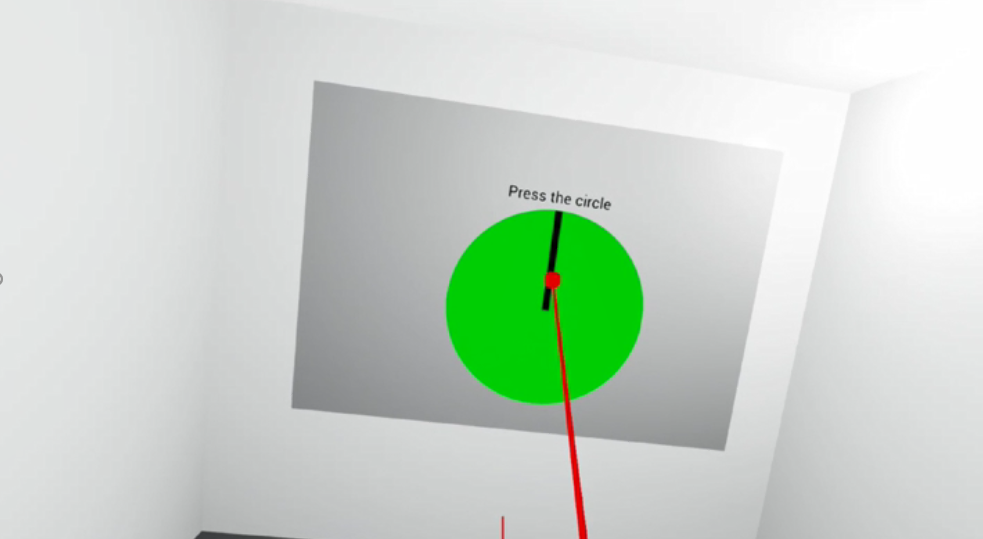
\includegraphics[width=\textwidth]{Images/Boredom.png} 
\caption{ Bild des Langeweile-Szenarios in VR. }
\label{fig:boredom4} 
\end{figure}

